\apendice{Plan de Proyecto Software}
\section{Introducción}
Este documento tiene como objetivo una presentación de manera integral de todos los aspectos clave relacionados con el desarrollo y la implementación del proyecto. 

Para realizar un correcto desarrollo del proyecto, se ha definido una planificación temporal y se desarrollará una planificación económica para saber el coste aproximado total del producto desarrollado.
\section{Planificación temporal}
El proyecto se ha desarrollado a lo largo de un total de 14 semanas (aproximadamente 4 meses), durante las cuales se ha distribuido el trabajo de forma progresiva. 

En la \textit{tabla \ref{fig:Planificación}} se puede observar un resumen de la planificación temporal.
\begin{figure}[h]
        \centering
        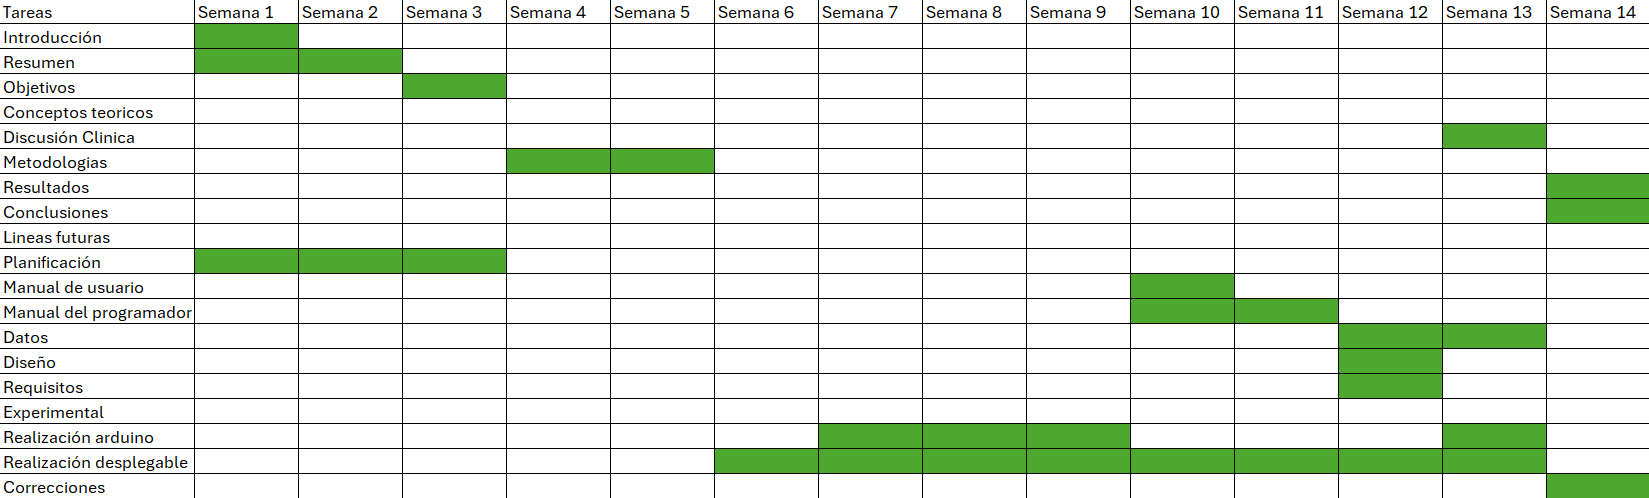
\includegraphics[width=1.25\textwidth]{img/planificación.png}
        \caption{Planificación del proyecto. Fuente propia}
        \label{fig:Planificación}
    \end{figure}

\section{Planificación económica}

La planificación económica consiste en el análisis total del precio del proyecto, incluyendo de manera individual los precios de los componentes del dispositivo (hardware), software y personal.

En la tabla \ref{tab:Costes Totales}, se puede observar el precio total del proyecto. Todos los precios han sido obtenidos en 2025, por lo cual el coste puede variar en un futuro. 

\subsection{Precios Hardware}
Para calcular el precio total de los costes de los materiales del dispositivo, se tiene en cuenta la suma total de los precios de los componentes, así como una suma de los gastos de producción y un porcentaje destinado a los beneficios. 

En la tabla \ref{tab:costes_hardware} se ha realizado un resumen de gastos y precio total. 
\begin{table}[]
\centering
\begin{tabular}{|l|p{8cm}|l|}
\hline
\rowcolor[HTML]{BFBFBF} 
\textbf{} & \textbf{Cálculos} & \textbf{Precio} \\ \hline
Gastos de los componentes & Suma total de los precios de los componentes del dispositivo & 61,7€\\ \hline
Gastos de producción & 10\% del precio de los
 componentes & 6,17€\\ \hline
Ingresos destinados a beneficio & 15\% de los gastos totales & 10,18€\\ \hline
\textbf{Total}& Suma total de los gastos & 78,05€ \\ \hline
\end{tabular}
\caption{Costes de dispositivos hardware.}
\label{tab:costes_hardware}
\end{table}

\subsubsection{\textbf{Desglose de precios de los componentes}}
Los precios de cada componente han sido seleccionados, siendo los mínimos encontrados en el mercado de páginas oficiales.
\begin{itemize}
    \item Placa Elegoo+USB: 15,99€
    \item Resistencias: 7*0,01299€= 0.091€
    \item Sensores de fuerza: 5*8,1€= 40,5€
    \item Elementos conectores (cables dupont): 29*0,07€=2.03€
    \item Protoboard: 2,83€
    \item Luz y botón: 0,20€
\end{itemize}
No se han contemplado los gastos de la compra de un ordenador, ya que en la actualidad en toda área del hospital se cuenta con uno de forma habitual. 

\subsubsection{Mango}

Para complementar con el desarrollo del proyecto, se ha diseñado un mango (véase \textit{Figuras} \ref{fig:Visión 1 del Mango.} \ref{fig:Visión 2 del Mango} \ref{fig:Visión 3 del Mango}) donde colocar los sensores. Diseñado especialmente para ser utilizado con la tabla canadiense. 

Está diseñado con la aplicación FreeCAD. Sus dimensiones son 60x60x135 mm. Cuenta con un agujero interior para insertar una de las barras de la tabla canadiense. 
Además, tiene cinco hendiduras destinadas a situar cada uno de los sensores.

\begin{figure}
    \centering
    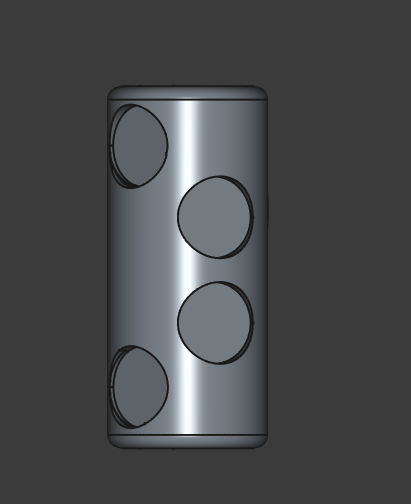
\includegraphics[width=0.35\linewidth]{img/Mango1.png}
    \caption{Visión 1 del Mango. Fuente propia}
    \label{fig:Visión 1 del Mango.}
\end{figure}
\begin{figure}
    \centering
    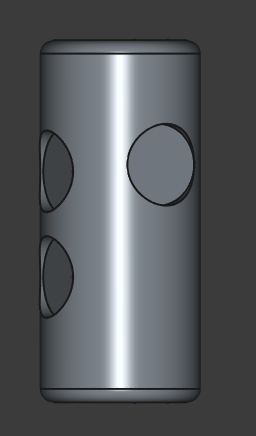
\includegraphics[width=0.25\linewidth]{img/Mango2.png}
    \caption{Visión 2 del Mango. Fuente propia}
    \label{fig:Visión 2 del Mango}
\end{figure}
\begin{figure}
    \centering
    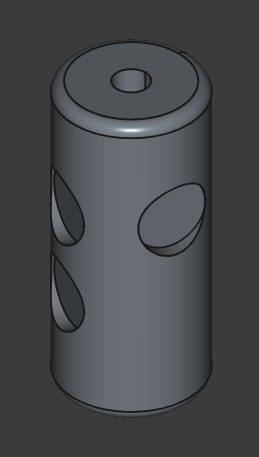
\includegraphics[width=0.25\linewidth]{img/Mango3.png}
    \caption{Visión 3 del Mango. Fuente propia}
    \label{fig:Visión 3 del Mango}
\end{figure}

Para tener este producto en físico, se ha pensado en la impresión 3D. Los costes de dicho accesorio difieren según donde y como se realice la impresión. 
Se ha considerado dos presupuestos diferentes según el método de impresión:
\begin{enumerate}
    \item Impresión propia: he seleccionado la impresora Ender-3 V3 SE \cite{Ender-3}, con un precio de 169 € y un filamento PLA\cite{PLA}, con un precio de 20,99 € el Kg. 
    \item Impresion mediante una empresa externa: he seleccionado la empresa ErreBiLAB \cite{ErreBiLAB}, ya que ofrece el precio más bajo de los que he visto disponibles. El precio de una pieza es de 41,03 €, este precio se va disminuyendo según el volumen de encargos. 
\end{enumerate}

La tabla \ref{tab:Impresión} resume lo que supondría esta adicción al prototipo (por cada mango), teniendo en cuenta la fabricación de 10 mangos. 
Ambas impresiones tienen los mismos requisitos.
\begin{table}[h] 
    \centering
    \begin{tabular}{|l|l|}
    \hline
    \rowcolor[HTML]{BFBFBF} 
    \textbf{Impresión propia} & \textbf{Imprimir mediante un 3º} \\ \hline
     17,6€ & 37€  \\ \hline
    \end{tabular}
    \caption{Costes de impresión}
    \label{tab:Impresión}
\end{table}

\subsection{Precios software}
No se incluye ningún gasto en software ya que todo el material utilizado es gratuito y de código abierto.

\subsection{Precio de personal}
Para calcular el salario del personal se ha partido de los datos publicados de salarios de ingenieros biomédicos, profesionales con un perfil técnico y formativo parecido al de un ingeniero de la salud.
Actualmente, en España el sueldo medio de un ingeniero biomédico es de 3.500€ \cite{SueldoBioing}\footnote{Página web de indeed, donde se puede ver sueldos de diferentes trabajos \cite{SueldoBioing}.}\cite{SUELDO}. Este sueldo es más bajo en recién egresados suponiendo un sueldo aproximado entre 1.500€ y 1.900€ mensuales.\cite{Sueldo_egresado}\footnote{Página web de la UAX con información económica sobre el salario de un graduado en ingeniería biomédica \cite{Sueldo_egresado}.}.


En la tabla \ref{tab:costes_personal} se recoge el sueldo aproximado que debería cobrar por el proyecto un ingeniero de la salud.

\begin{table}[h]
\centering
\begin{tabular}{|l|l|}
\hline
\rowcolor[HTML]{BFBFBF} 
\textbf{} & \textbf{Precio} \\ \hline
Sueldo mensual & 1.600€ \\ \hline
\textbf{Total en 4 meses }& 6.400€ \\ \hline
\end{tabular}
\caption{Costes de sueldos del personal brutos.}
\label{tab:costes_personal}
\end{table}

\begin{table}[h]
\centering
\begin{tabular}{|l|l|}
\hline
\rowcolor[HTML]{BFBFBF} 
\textbf{} & \textbf{Precio} \\ \hline
Material & 78,05€ \\ \hline
Sueldo  &  6.400€ \\ \hline
\textbf{Total }& 6.478,05€ \\ \hline
\end{tabular}
\caption{Precio total del proyecto}
\label{tab:Costes Totales}
\end{table}

\section{Viabilidad legal}
Se debe tener en cuenta la normativa legal desde la creación de la idea hasta la comercialización y uso postventa.

Es esencial la implementación de leyes que garanticen el cumplimiento de la normativa aplicable que respalde los derechos y obligaciones del autor. Incluyendo desde leyes de las regulaciones técnicas, de propiedad intelectual y de responsabilidad profesional, conforme a lo establecido en la legislación.

Asimismo, se deben implementar medidas vigorosas que protejan la integridad de los usuarios y la confidencialidad de sus datos. 

Podemos dividir el proceso en 2 fases, la primera fase incluiría la creación de la idea, diseño, desarrollo y realización de pruebas, y una segunda fase que incluya la comercialización y postventa.

\subsection{1º Fase}

Durante la primera fase de creación de la idea, diseño, desarrollo y realización de las pruebas, se deberán tener en cuenta las siguientes normas legislativas: 

\begin{itemize}
    \item Ley 24/2015, de 24 de julio \cite{boe--2015-8328}, de Patentes: Establece los derechos, requisitos y procedimientos para obtener una patente y reforzar la seguridad jurídica. Esta última versión simplifica y agiliza el procedimiento.
    \item Real Decreto Legislativo 1/1996, de 12 de abril,\cite{boe--1996-8930} sobre la Ley de la Propiedad Intelectual: Establece los derechos de una obra al autor solo por el hecho de crearlo. 
    \item Real Decreto 192/2023, de 21 de marzo \cite{ministerio_de_sanidad_real_2023}, por el que se regulan los productos sanitarios. 
    \item UNE-EN 60601-1:2008 \cite{UNE2008}, norma que regula los requisitos generales para la seguridad básica y funcionamiento esencial de equipos electromédicos.
    \item UNE-EN ISO 14971:2020 \cite{UNE2020}, norma para la gestión de riesgos de dispositivos médicos.
\end{itemize}


\subsection{2º Fase}
La segunda fase de comercialización y postventa se deberá desarrollar según las siguientes normas legislativas: 
\begin{itemize}
    \item Ley 3/1991, de 10 de enero \cite{boe--1991-628}, de Competencia Desleal, sobre la promoción y comercialización del producto, realizando una publicidad lícita, veraz y no engañosa.
    \item Ley Orgánica 3/2018, de 5 de diciembre \cite{boe--2018-16673}, de Protección de Datos Personales y garantía de los derechos digitales.
    \item Reglamento (UE) 2016/679 del Parlamento Europeo y del Consejo, de 27 de abril de 2016 \cite{boees}, relativo a la protección de las personas físicas en lo que respecta al tratamiento de datos personales y a la libre circulación de estos datos.
    \item Ley 29/2006, de 26 de julio \cite{boe--2006-13554}, de garantías y uso racional de los medicamentos y productos sanitarios.
\end{itemize}